\usetikzlibrary{calc}
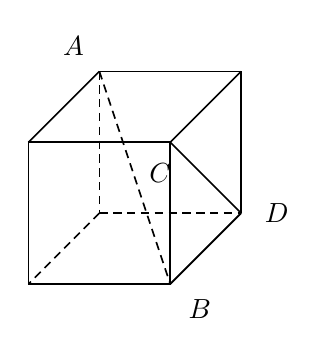
\begin{tikzpicture}[x=1cm,y=1cm,line width=.6pt,font=\normalsize]
% cube: front face FFL,FBR,FTR,FTL ; back face offset
\coordinate (FFL) at (0,0);
\coordinate (FBR) at (1.8,0);
\coordinate (FTR) at (1.8,1.8);
\coordinate (FTL) at (0,1.8);
\coordinate (BBL) at (0.9,0.9);
\coordinate (BRB) at (2.7,0.9);
\coordinate (BTR) at (2.7,2.7);
\coordinate (A) at (0.9,2.7);
\coordinate (C) at (1.8,1.8);
\coordinate (B) at (1.8,0);
\coordinate (D) at (2.7,0.9);
% front face solid
\draw (FFL) -- (FBR) -- (FTR) -- (FTL) -- cycle;
% outer/back outline solid
\draw (FFL) -- (FTL);
\draw (FTL) -- (A);
\draw (A) -- (BTR);
\draw (BTR) -- (D);
\draw (FBR) -- (D);
% top face edges solid
\draw (A) -- (BTR);
\draw (BTR) -- (C);
\draw (C) -- (FTL);
% right-face bottom depth solid, diagonal CD solid
\draw (FBR) -- (D);
\draw (C) -- (D);
% front-right vertical is C-B (cube edge, solid, coincides with front face)
% hidden dashed: A-B space diagonal, A-BBL, BBL-FFL, BBL-D
\draw[densely dashed] (A) -- (B);
\draw[densely dashed] (A) -- (BBL);
\draw[densely dashed] (BBL) -- (FFL);
\draw[densely dashed] (BBL) -- (D);
% labels with clearance
\node[anchor=south east,xshift=-2pt,yshift=2pt] at (A) {$A$};
\node[anchor=north east,xshift=4pt,yshift=-4pt] at (C) {$C$};
\node[anchor=north west,xshift=3pt,yshift=-2pt] at (B) {$B$};
\node[anchor=west,xshift=5pt,yshift=0pt] at (D) {$D$};
\end{tikzpicture}
